\documentclass[a4paper,
               %boxit,
               %titlepage,   % separate title page
               %refpage      % separate references
              ]{jacow}

\makeatletter%
	\ifboolexpr{bool{xetex}}
	 {\renewcommand{\Gin@extensions}{.pdf,%
	                    .png,.jpg,.bmp,.pict,.tif,.psd,.mac,.sga,.tga,.gif,%
	                    .eps,.ps,%
	                    }}{}
\makeatother

 {\usepackage[utf8]{inputenc}}           % switch to utf8

\ifboolexpr{bool{xetex} or bool{luatex}} % test for XeTeX/LuaTeX
 {}                                      % input encoding is utf8 by default


\usepackage[USenglish]{babel}			 
\usepackage{tikz-palattice}
\usepackage[final]{pdfpages}
\usepackage{multirow}
\usepackage{ragged2e}
\usepackage{placeins}
\usepackage{subcaption}
%
% if BibLaTeX is used
%
\ifboolexpr{bool{jacowbiblatex}}%
 {%
  \addbibresource{jacow-test.bib}
  \addbibresource{biblatex-examples.bib}
 }{}
\listfiles

%
% command for typesetting a \section like word
%
\newcommand\SEC[1]{\textbf{\uppercase{#1}}}
\newcommand*{\matr}[1]{\mathbf{#1}}
\newcommand{\specialcell}[2][c]{%
  \begin{tabular}[#1]{@{}c@{}}#2\end{tabular}}
%%
%%   Lengths for the spaces in the title
%%   \setlength\titleblockstartskip{..}  %before title, default 3pt
%%   \setlength\titleblockmiddleskip{..} %between title + author, default 1em
%%   \setlength\titleblockendskip{..}    %afterauthor, default 1em

%\copyrightspace %default 1cm. arbitrary size with e.g. \copyrightspace[2cm]

% testing to fill the copyright space
%\usepackage{eso-pic}
%\AddToShipoutPictureFG*{\AtTextLowerLeft{\textcolor{red}{COPYRIGHTSPACE}}}

\begin{document}

\title{Compact ring-based X-ray source with
on-orbit and on-energy laser-plasma
injection}

\author{Marlene Turner \textsuperscript{1} \thanks{marlene.turner@cern.ch}, CERN, Geneva, Switzerland\\
Jeremy Cheatam, Auralee Edelen, CSU, Fort Collins, Colorado, USA \\
Osip Lishilin, DESY Zeuthen, Zeuthen, Germany\\
Aakash Ajit Sahai, Imperial College Physics, London, Great Britain\\
Andrei Seryi, JAI, Oxford, Great Britain\\
Brandon Zerbe, MSU, East Lansing, Michigan\\
Andrew Lajoie, Chun Yan Jonathan Wong, NSCL, East Lansing, Michigan\\
Kai Shih, SBU, Stony Brook, New York\\
James Gerity, Texas A\&M University, College Station\\
Gerard Lawler, UCLA, Los Angeles, California\\
Kookjin Moon, UNIST, Ulsan, Korea\\
		\textsuperscript{1}also at Technical University of Graz, Graz, Austria}
	
\maketitle

%
\begin{abstract}
We report here the results of a one week long investigation into the conceptual design of an X-ray source based on a compact ring with on-orbit and on-energy laser-plasma acceleration injection (mini-project 10.4 from \cite{UNIFYINGPHYSICS}) performed during the June 2016 USPAS class "Physics of Accelerators, Lasers, and Plasma\ldots". We describe three versions of the light source with the constraints of the electron beam with energy $1\,\rm{GeV}$ or $3\,\rm{GeV}$ and a lattice bending magnetics being normal (only for the $1\,\rm{GeV}$ beam) or superconducting (for either beam).  We describe the design choices, present relevant parameters, and describe insights into such machines.
\end{abstract}


\section{INTRODUCTION}

Due to the high accelerating gradients that can be achieved using plasma, combining the field of Laser wakefield acceleration (LWFA) with synchrotron light production offers the possibility of creating compact accelerators and light sources.
We sought to outline a design for a compact synchrotron light source that produces \SI{0.4}{keV} (water-window) or \SI{10}{keV} photons using such acceleration technology. We estimate the design parameters of the compact light source, the achievable brilliance, and we discuss the feasibility and challenges of the design. 

We assume the presence of state of the art technology including a laser plasma gas-jet accelerator, a quadrupole doublet to focus and confine the beam, four 90 degree dipole bending magnets (super-conducting or normal conducting) to keep the beam on a periodic lattice, and a \SI{2}{m} long wiggler magnet to produce the desired radiation. A schematic of the design is in Fig. \ref{schematics}, and investigated designs criteria are detailed below: 
\begin{itemize}
\item \SI{0.4}{keV} photons produced by a \SI{1}{GeV} electron beam and normal-conducting magnets.
\item \SI{0.4}{keV} photons produced by a \SI{1}{GeV} electron beam and super-conducting magnets.
\item \SI{10}{keV} photons produced by a \SI{3}{GeV} electron beam and super-conducting magnets.
\end{itemize}

\section{DESIGN OF THE MACHINE}
\subsection{Plasma based electron injector}

The laser wakefield acceleration and injection stage provides the electron beam for the compact ring. An intense laser pulse from a Ti:Sapphire laser is injected through a window in one of the bending dipoles, impinges on a gas jet, ionizes the plasma, and creates strong plasma wakefields inject electrons from the background plasma and accelerate them. The chosen laser and plasma parameters are summarized in Tables \ref{laserparameters} and \ref{plasmaparameters}.
Based on existing systems, we choose laser parameters achievable in the near future. A Ti:Sapphire laser system with a laser wavelength of $\lambda_l = 780\,\rm{nm}$, a pulse duration of $50\,\rm{fs}$, a maximum laser power of $400\,\rm{TW}$, $20\,\rm{J}$ of energy per pulse, and a laser spot size of $3.8\,\rm{nm}^2$ \cite{LASER}. The laser intensity $I$ is then approximately $9.9\cdot10^{18}\,\rm{W/cm}^2$ which corresponds to an $a_0$ of about $2.1$ for a Gaussian radial laser distribution. 
\begin{equation}
a_0 \approx \left( \frac{I [\rm{W/cm}^2]}{1.37e18} \right) ^{\frac{1}{2}} \cdot \lambda_l[\mu\rm{m}]
\end{equation}
The chosen plasma density of the gas-jet is $n = $\SI{1.75e17}{cm^{-3}} and optimizes the achievable maximum electron energy. The laser frequency was confirmed to be greater than the critical plasma frequency $\omega_c$ [reference]
\begin{equation}
\omega_c = \frac{n^2}{4 \pi c^2 r_e}
\end{equation}
where $c$ is the speed of light and $r_e$ is the classical electron radius.

The depletion $L_{dpl}$ and dephasing length $L_{dph}$ for this injector system are estimated with: 
\begin{equation}
L_{dpl} = \frac{1}{2 a_0} \frac{\lambda_p^3}{\lambda_l^2}\, , 
L_{dph} = \frac{1}{2} \frac{\lambda_p^3}{\lambda_l^2}
\end{equation}

to be $L_{dpl}\approx 17\,\rm{cm}$ and $L_{dph}\approx 35\,\rm{cm}$, thus $17\,\rm{cm}$ is the upper bound on our total possible acceleration length. The maximum accelerating gradient $E_{max}$ is estimated with
\begin{equation}
eE_{max} = 1 \frac{\rm{eV}}{\rm{cm}} \cdot n^{1/2}[\rm{cm}^{-3}]
\end{equation}
to be \SI{420}{MeV/cm}.
This means that our target energies of $1\,\rm{GeV}$ and $3\,\rm{GeV}$ can be reached with an acceleration length of $2.4\,\rm{cm}$ and $7.2\,\rm{cm}$. This acceleration length is longer than gas jets in use presently and may require a novel gas jet setup [references?], particularly for the $3\,\rm{GeV}$ beam.

In this design, we are relying on analytic estimates rather than the results of 3D simulations of the setup. Consequently, for the remainder of the ring calculations we used electron beam parameters that are typically achievable with similar laser wakefield acceleration stages [reference]. The chosen electron beam size is $\sigma_r \approx 1 \frac{c}{\omega_p} \approx 12 \mu\rm{m}$, the electron energy spread is $\frac{\Delta E}{E_0} = 2\%$, and the electron beam divergence is $\sigma_\theta = 0.5\,\rm{mrad}$. Reasonable bunch charge for the \SI{1}{GeV} and \SI{3}{GeV} electron beams are \SI{10}{pC} and \SI{7}{pC}.
\begin{table}[hbt]
%   \vspace*{-.5\baselineskip}
   \centering
   \caption{Laser parameters of the plasma injector}
   \begin{tabular}{lc}
       \toprule
Laser wavelength & \SI{780}{nm}\\
Laser power & \SI{379}{TW}\\
Spot size &  \SI{3.8e-9}{m^2} \\
Intensity & \SI{9.9e18}{W/cm^2} \\
a\_0 & \SI{2.1}{} \\
Laser pulse length (FWHM) & \SI{50}{fs} \\
Reprate &  	$\sim$\SI{1}{Hz} \\
Pulse Energy & \SI{20}{J} \\
       \bottomrule
   \end{tabular}
   \label{laserparameters}
%   \vspace*{-\baselineskip}
\end{table}

\begin{table}[hbt]
%   \vspace*{-.5\baselineskip}
   \centering
   \caption{Plasma parameters}
   \begin{tabular}{lc}
       \toprule
Plasma density & \SI{1.75e17 }{cm^-3}\\
Plasma wavelength &  \SI{76}{\micro m} \\
Plasma frequency & \SI{3.97e12}{Hz} \\
Plasma angular frequency & \SI{2.49e13}{s^-1} \\
Accelerating gradient & \SI{0.42}{GeV/cm} \\
Bubble size &  \SI{38}{\micro m} \\
Depletion length & \SI{16.9}{cm} \\
Dephasing length & \SI{33.5}{cm} \\
Acceleration length for 1 GeV & \SI{2.4}{cm} \\
Acceleration length for 3 GeV & \SI{7.2}{cm} \\
       \bottomrule
   \end{tabular}
   \label{plasmaparameters}
%   \vspace*{-\baselineskip}
\end{table}

\subsection{Magnet Design}
The design of the compact ring (see Figure \ref{schematics}) is laid out as four $90\,\rm{-degree}$ sector dipoles, either \SI{10}{T} super-conducting (s.c.) or \SI{1.5}{T} normal conducting (n.c.). Parameters for the bending magnets are shown in Table \ref{magnets}. The laser-plasma injection system is located in the middle of a \SI{2}{m} drift, enclosed by a pair of focusing quadrupole doublets (strengths $\sim$ \SI{50}{T/m}, \SI{100}{T/m}) used to begin transport of the diverging electron beam born from the laser wakefield injector. 
The focusing strengths of the quadrupole magnets were calculated to parallelize  an electron beam with a radial size $\sigma_r = 12\,\mu\rm{m}$ and a divergence of $0.5\,\rm{mrad}$. Dipole magnets provide weak focusing, which is employed to compensate for space-charge effects.
The wiggler is located in the drift space opposing the injector, and the remaining two drift spaces are each \SI{0.5}{m} leaving enough space for limited diagnostics and collimators. The electron energy loss per turn is dominated by the synchrotron radiation loss $E_{sr}$ in the bending magnets. 
There is no accelerating section in our compact ring design. This means that the number of turns $N_{turns}$ is limited by the energy loss and the \SI{10}{cm} horizontal apertures of the bending magnets.
The number of turns was calculated by taking the radial electron beam size ($\sigma_r$), including energy spread and an covservative engineering fudge factor of 2, and calculating how much energy can be lost before the beam touches the aperture.

\begin{table}[hbt]
%   \vspace*{-.5\baselineskip}
   \centering
   \caption{Dipole bending magnet parameters}
   \begin{tabular}{lccc}
       \toprule
\textbf{Parameter} & \textbf{\SI{1}{GeV} n.c.} & \textbf{\SI{1}{GeV} s.c.} & \textbf{\SI{1}{GeV} s.c.}\\
Bend. strength & 1.5 T & 10 T m & 10 T\\
Bend. radius & 2.23 m & 0.84 m & 1.02 m\\
Circumf. & 19.1 m & 7.1 m & 9.4 m\\
$E_{sr}$/turn & 40 keV & 260 keV & 7 MeV\\
$N_{turns}$ & 62 & 490 & 13\\
       \bottomrule
   \end{tabular}
   \label{magnets}
%   \vspace*{-\baselineskip}
\end{table}

%The table was moved from its original position because otherwise it ends up at the end of the document. (Try it if you dont believe me ;) )
\begin{table*}[tb!]
  \centering
  \caption{Chosen (first box) and derived (second box) parameters detailing X-ray source. }
  \label{tab:radiation}
  \begin{tabular}{cccc}
    \hline
    $\text{E}_\text{electron} (\text{GeV})$ &  $1.0$ & $1.0$ & $3.0$ \\
    $\text{B}_\text{turn} (\text{T})$ & $1.5$ & $10.0$ & $10.0$ \\
    $\text{E}_\text{photon}$ (\text{keV}) & $0.4$ & $0.4$ & $10.0$ \\
    $\lambda_\text{wiggler}$ (\text{mm}) & $15$ & $15$ & $100$ \\
    \hline
    $\text{B}_\text{wiggler} (\text{T})$ & $0.60$ & $0.60$ & $1.7$ \\
    $\text{K}$ & $0.84$ & $0.84$ & $16$ \\
    $\text{E}_\text{radiated} (\text{keV})$ & $2.1$ & $2.1$ & $140$ \\
    $\text{Brilliance per electron lifetime} \left ( \frac{\text{photons}}{\text{mm}^2 \text{mrad}^2 \text{sec}} \right )$ & $1.8 \times 10^{10}$ & $91  \times 10^{10}$ & $1.3  \times 10^{10}$ \\
    $\text{Brilliance per spill} \left ( \frac{\text{photons}}{\text{mm}^2 \text{mrad}^2 \text{sec}} \right )$& $4.7 \times 10^{15}$ &  $78 \times 10^{15}$ & $27  \times 10^{15}$ \\
    $\text{x-ray train duration} ( \mu\text{sec})$ & $3.9$ & $12$ & $0.47$\\
    \hline 
  \end{tabular}
\end{table*}



\begin{figure}
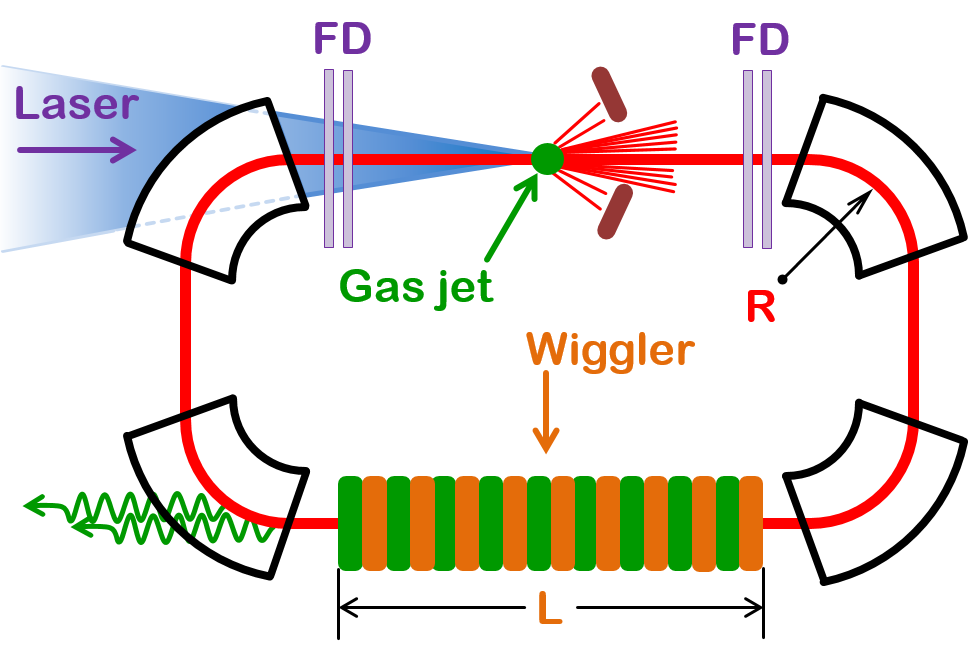
\includegraphics[width = 0.5\textwidth]{on-orbit-laser-plasma-2.png}
\caption{Schematics of the compact ring design. The laser beam enters through a window in the B4 dipole bending magnet, ionizes the gas jet and creates strong plasma wakefields to self-inject and accelerate electrons. Furthermore the produced electron beam gets focused with a quadrupole doublet. The electron beam is held on a circular trajectory by four 90-degree bending magnets (B1-B4). Opposite to the plasma injector, a Wiggler magnet produces the desired radiation.}
	\label{schematics}
\end{figure}

\subsection{Production of Radiation}
\label{radiation}
Table \ref{tab:radiation} details the radiation source parameters for all considered design versions.  A standard length of \SI{2}{m} was chosen for the undulating magnetic field region, where the electron bunch emits an approximately \SI{6.7}{ns}-long X-ray pulse at each turn until it is scraped by the apertures. As can be seen in the table, X-ray energy was designed to either be within the water window ($0.4\,\text{keV}$) or to be fairly hard ($10\,\text{keV}$) depending on the energy of the injected electron pulse.  The chosen parameters result in the source being near the wiggler/undulator transition or well within the wiggler regime, respectively, as can be seen by the parameter K.  Of the chosen parameter sets, the \SI{1}{GeV} electrons with the superconducting bending magnets (\SI{10}{T}) resulted in the largest brightness.




\section{DISCUSSION}

One worrying design issue is that the gas/plasma from the injector resides in the lattice longer than it takes the electron beam to make circle the lattice. The gas flow velocity from typical gas jets is $M = 20\,\rm{km/s}$ \cite{GASFLOW}, and one electron beam turn in a \SI{10}{m} circumference ring takes $\sim$ \SI{30}{ns}.  Thus the gas flow advances by $\sim$\SI{600}{$\mu$m} and will therefore still be in the path of the beam for much of its residence time. Taking $10^{14}\,\rm{W/cm}^2$ as ionization threshold of the plasma and assuming a radial laser size of \SI{35}{$\mu$m} gives a plasma channel radius of \SI{143} {$\mu$m}. This estimate suggest that the plasma column has already propagated far enough to eliminate the possibility of any further interaction with the beam. So, the electron beam is only likely to interact with the residual gas and not the laser-ionized plasma column. Thus, the interaction process of the beam is dominated by random scattering off the gas, which leads to a divergence growth of the order of micro-rad, as opposed to a coherent lensing of the order of milli-rad by the plasma [2]. It is unlikely that an electron beam with pC charge with a beam size of $\sigma_r = 5\mu\rm{m}$ and $\sigma_z = 10\,\mu\rm{m}$ ionizes gas.\\
Apart from using the radiation created by the wiggler, it would also be possible to use the radiation from the bending magnets or the X-rays produced by the betatron oscillations of the electron beam in the bubble. The latter has already been considered by \cite{PRODKEVS}
A Compton light source could be realized by making the electron bunch collide with a laser pulse.
\section{CONCLUSIONS}

In this report we propose different design solutions for a compact ring-based X-ray source with an on-orbit and on-energy laser-plasma injector. We consider four 90 degrees bending magnets to keep the particles on a circular orbit, the electrons are self-injected and accelerated by the plasma wakefield of a gas-jet excited by a \SI{400}{TW} laser system, and the desired radiation is created by a wiggler magnet. The peak brilliance is calculated in the section 'Production of Radiation' and reaches up to $7.8e16\,\rm{photons/(mm}^2 \rm{mrad}^2)$. Even though modern light sources routinely create a peak brilliance in the order of $10^{25}\,\rm{photons/(mm}^2 \rm{mrad}^2 0.1\%\rm{BW})$ \cite{DESY}, this design can be considered attractive due to its compactness and small footprint. This design would be suitable for use in, for example, a university setting.
Future work should include plasma simulations to obtain better estimates for the electron beam parameters, optics simulations and particle tracking to obtain electron beam sizes, studies on the gas-jet design, further investigations on the electron scattering on the residual gas, and a more detailed description of the magnet design.   


\begin{thebibliography}{99}
\bibitem{UNIFYINGPHYSICS} Unifying physics of accelerators, lasers and plasma, A. Seryi, CRC Press, 2015.

\bibitem{LASER} Ultra-high intensity- 300-TW laser at 0.1 Hz repetition rate., Opt. Express 3, 2109--2114 (2008); doi: 10.1364/OE.16.002109

\bibitem{GASFLOW} High density gas jet nozzle design for laser target production, Review of Scientific Instruments 72, 2961 (2001); doi: 10.1063/1.1380393

\bibitem{BPINTER}Beam interaction with Plasma-Vacuum interface, CLIC Experimental \& Breakdown Studies Meeting, August 2013 

\bibitem{DESY} DESY Photon science

%\bibitem{PRODRAD} Albert, F., et al. "Full characterization of a laser-produced keV x-ray betatron source." Plasma Physics and Controlled Fusion 50.12 (2008): 124008.

\bibitem{SYNCHRRAD} Schlenvoigt, Hans-Peter. "Synchrotron radiation sources driven by laser-plasma accelerators." (2009). 

\bibitem{PRODKEVS} Rousse, Antoine, et al. "Production of a keV X-ray beam from synchrotron radiation in relativistic laser-plasma interaction." Physical review letters 93.13 (2004): 135005.



\end{thebibliography}
\end{document}

    Contact GitHub API Training Shop Blog About 

    © 2016 GitHub, Inc. Terms Privacy Security Status Help 

